\exercise

Given the undirected and weighted graph  $$G = \big\{ (A,B,2),\ (A,F,4),\ (A,E,6),\
(B,C,1),\ (B,F,3),\ (C,D,3),\ (C,F,5) \big\}\ ,$$ compute the MST via the
external-memory algorithm of Sibeyn switching to Kruskal when the graph consists
of 3 nodes (hence $M$ is able to host 3 nodes).

\solution

Let us reassign to all nodes a numeric label corresponding to the rank of its
letter, such as $A \mapsto 1,\ \dots,\ F \mapsto 6$. Then we apply the random
permutation $\pi(n) = \left( 3n + 2 \bmod 7 \right) + 1$, which produces the
following mapping $$\pi(A \mapsto 1) = 6,\ \pi(B \mapsto 2) = 2,\ \pi(C \mapsto
3) = 5,\ \pi(D \mapsto 4) = 1,\ \pi(E \mapsto 5) = 4,\ \pi(F \mapsto 6) = 7\ .$$
We can now proceed constructing the tuples for the priority queue and execute
the Sibeyn's algorithm, starting with $current = 0$ and extracting the minimum
entry in the priority queue $Q$ (\autoref{fig:sibeyn0}), ordered by the first
and third entry:
%
\begin{enumerate}
  \item {\bf extract} $\langle 1,5,3,C,D \rangle,\ current \neq 1 \implies current \gets 1,\ relinkTo \gets 5$, {\bf output} $(C,D,3)$.
  \item {\bf extract} $\langle 2,5,1,B,C \rangle,\ current \neq 2 \implies current \gets 2,\ relinkTo \gets 5$, {\bf output} $(B,C,1)$.
  \item {\bf extract} $\langle 2,6,2,A,B \rangle,\ current = 2,\ relinkTo \neq 6 \implies\ $ {\bf insert}  $\langle 5,6,2,A,B \rangle$.
  \item {\bf extract} $\langle 2,7,3,B,F \rangle,\ current = 2,\ relinkTo \neq 7 \implies\ $ {\bf insert}  $\langle 5,7,3,B,F \rangle$.
  \item {\bf extract} $\langle 4,6,6,A,E \rangle,\ current \neq 4 \implies current \gets 4,\ relinkTo \gets 6$, {\bf output} $(A,E,6)$.
  \item {\bf extract} $\langle 5,6,2,A,B \rangle,\ current \neq 5,\ |N| = 3 \implies $ {\bf stop}.
\end{enumerate}
%
We now sort the remaining edges by their cost and conclude using Kruskal's
algorithm, starting from the subforests $S = \left\{\{5\},\ \{6\},\ \{7\}\right\}$:
%
\begin{enumerate}
  \item {\bf extract} $\langle 5,6,2,A,B \rangle,\ \text{\sc FindSet}(5) \neq \text{\sc FindSet}(6) \implies S \gets \left\{\{5,\ 6\},\ \{7\}\right\}$, {\bf output} $(A,B,2)$.
  \item {\bf extract} $\langle 5,7,3,B,F \rangle,\ \text{\sc FindSet}(5) \neq \text{\sc FindSet}(7) \implies S \gets \left\{\{5,\ 6,\ 7\}\right\}$, {\bf output} $(B,F,3)$.
  \item {\bf extract} $\langle 6,7,4,A,F \rangle,\ \text{\sc FindSet}(6) = \text{\sc FindSet}(7) \implies $ {\bf pass}.
  \item {\bf extract} $\langle 5,7,5,C,F \rangle,\ \text{\sc FindSet}(5) = \text{\sc FindSet}(7) \implies $ {\bf pass}.
\end{enumerate}
%
\begin{figure}
  \begin{subfigure}{\linewidth}
    \hspace{0.1\linewidth}%
    \begin{subfigure}[m]{0.4\linewidth}
      \centering
      \begin{tabular}{|c|c|c|c|c|}
        \hline
        $\min\pi$ & $\max\pi$ & $c(u,v)$ & $u$ & $v$ \\ \hline\hline
        1 & 5 & 3 & $C$ & $D$ \\ \hline
        2 & 5 & 1 & $B$ & $C$ \\ \hline
        2 & 6 & 2 & $A$ & $B$ \\ \hline
        2 & 7 & 3 & $B$ & $F$ \\ \hline
        4 & 6 & 6 & $A$ & $E$ \\ \hline
        5 & 7 & 5 & $C$ & $F$ \\ \hline
        6 & 7 & 4 & $A$ & $F$ \\ \hline
      \end{tabular}
    \end{subfigure}%
    \begin{subfigure}[m]{0.4\linewidth}
      \centering
      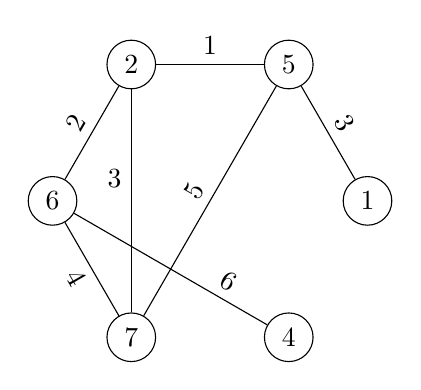
\begin{tikzpicture}
        \def \radius {2cm}

        \node[draw, circle] (A) at (180:\radius) {6};
        \node[draw, circle] (B) at (120:\radius) {2};
        \node[draw, circle] (C) at (60:\radius) {5};
        \node[draw, circle] (D) at (0:\radius) {1};
        \node[draw, circle] (E) at (300:\radius) {4};
        \node[draw, circle] (F) at (240:\radius) {7};

        \path (A) edge node[sloped, above] {2} (B);
        \path (A) edge node[sloped, below] {4} (F);
        \path (A) edge node[pos=0.75, sloped, above] {6} (E);
        \path (B) edge node[sloped, above] {1} (C);
        \path (B) edge node[pos=0.4, left] {3} (F);
        \path (C) edge node[sloped, above] {3} (D);
        \path (C) edge node[sloped, above] {5} (F);
      \end{tikzpicture}
    \end{subfigure}%
    \hspace{0.1\linewidth}

    \caption{Initial state.}
    \label{fig:sibeyn0}

  \end{subfigure}

  \vspace{1em}%
  \begin{subfigure}{\linewidth}
    \hspace{0.1\linewidth}%
    \begin{subfigure}[m]{0.4\linewidth}
      \centering
      \begin{tabular}{|c|c|c|c|c|}
        \hline
        $\min\pi$ & $\max\pi$ & $c(u,v)$ & $u$ & $v$ \\ \hline\hline
        2 & 5 & 1 & $B$ & $C$ \\ \hline
        2 & 6 & 2 & $A$ & $B$ \\ \hline
        2 & 7 & 3 & $B$ & $F$ \\ \hline
        4 & 6 & 6 & $A$ & $E$ \\ \hline
        5 & 7 & 5 & $C$ & $F$ \\ \hline
        6 & 7 & 4 & $A$ & $F$ \\ \hline
      \end{tabular}
    \end{subfigure}%
    \begin{subfigure}[m]{0.4\linewidth}
      \centering
      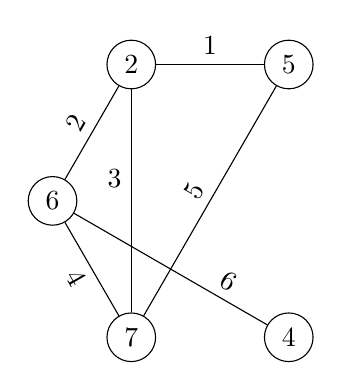
\begin{tikzpicture}
        \def \radius {2cm}

        \node[draw, circle] (A) at (180:\radius) {6};
        \node[draw, circle] (B) at (120:\radius) {2};
        \node[draw, circle] (C) at (60:\radius) {5};
        \node[draw, circle] (E) at (300:\radius) {4};
        \node[draw, circle] (F) at (240:\radius) {7};

        \path (A) edge node[sloped, above] {2} (B);
        \path (A) edge node[sloped, below] {4} (F);
        \path (A) edge node[pos=0.75, sloped, above] {6} (E);
        \path (B) edge node[sloped, above] {1} (C);
        \path (B) edge node[pos=0.4, left] {3} (F);
        \path (C) edge node[sloped, above] {5} (F);
      \end{tikzpicture}
    \end{subfigure}%
    \hspace{0.1\linewidth}

    \caption{State after step 1.}
    \label{fig:sibeyn1}

  \end{subfigure}

  \vspace{1em}%
  \begin{subfigure}{\linewidth}
    \hspace{0.1\linewidth}%
    \begin{subfigure}[m]{0.4\linewidth}
      \centering
      \begin{tabular}{|c|c|c|c|c|}
        \hline
        $\min\pi$ & $\max\pi$ & $c(u,v)$ & $u$ & $v$ \\ \hline\hline
        4 & 6 & 6 & $A$ & $E$ \\ \hline
        5 & 6 & 2 & $A$ & $B$ \\ \hline
        5 & 7 & 3 & $B$ & $F$ \\ \hline
        5 & 7 & 5 & $C$ & $F$ \\ \hline
        6 & 7 & 4 & $A$ & $F$ \\ \hline
      \end{tabular}
    \end{subfigure}%
    \begin{subfigure}[m]{0.4\linewidth}
      \centering
      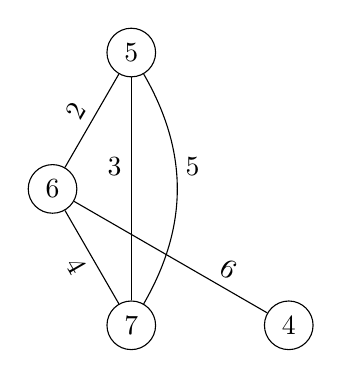
\begin{tikzpicture}
        \def \radius {2cm}

        \node[draw, circle] (A) at (180:\radius) {6};
        \node[draw, circle] (B) at (120:\radius) {5};
        \node[draw, circle] (E) at (300:\radius) {4};
        \node[draw, circle] (F) at (240:\radius) {7};

        \path (A) edge node[sloped, above] {2} (B);
        \path (A) edge node[sloped, below] {4} (F);
        \path (A) edge node[pos=0.75, sloped, above] {6} (E);
        \path (B) edge node[pos=0.4, left] {3} (F);
        \path (B) edge[bend left] node[pos=0.4, right] {5} (F);
      \end{tikzpicture}
    \end{subfigure}%
    \hspace{0.1\linewidth}

    \caption{State after step 4.}
    \label{fig:sibeyn4}

  \end{subfigure}

  \vspace{1em}%
  \begin{subfigure}{\linewidth}
    \hspace{0.1\linewidth}%
    \begin{subfigure}[m]{0.4\linewidth}
      \centering
      \begin{tabular}{|c|c|c|c|c|}
        \hline
        $\min\pi$ & $\max\pi$ & $c(u,v)$ & $u$ & $v$ \\ \hline\hline
        5 & 6 & 2 & $A$ & $B$ \\ \hline
        5 & 7 & 3 & $B$ & $F$ \\ \hline
        5 & 7 & 5 & $C$ & $F$ \\ \hline
        6 & 7 & 4 & $A$ & $F$ \\ \hline
      \end{tabular}
    \end{subfigure}%
    \begin{subfigure}[m]{0.4\linewidth}
      \centering
      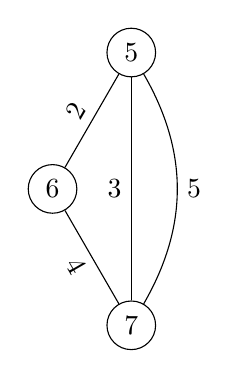
\begin{tikzpicture}
        \def \radius {2cm}

        \node[draw, circle] (A) at (180:\radius) {6};
        \node[draw, circle] (B) at (120:\radius) {5};
        \node[draw, circle] (F) at (240:\radius) {7};

        \path (A) edge node[sloped, above] {2} (B);
        \path (A) edge node[sloped, below] {4} (F);
        \path (B) edge node[left] {3} (F);
        \path (B) edge[bend left] node[right] {5} (F);
      \end{tikzpicture}
    \end{subfigure}%
    \hspace{0.1\linewidth}

    \caption{Final state.}
    \label{fig:sibeyn6}

  \end{subfigure}

  \caption{State of the graph and its priority queue $Q$ during the execution of
  Sibeyn's algorithm.}

  \label{fig:sibeyn}
\end{figure}
